\subsection{缓存驻留窗口的推导与逐事件分析}
\subsubsection{先进先出驻留窗口}
缓存时序候选需要判断一次顺序移动试图跨过哪个事件。考察张量 $t$ 成功填入后、首次淘汰前的一段驻留期，设其大小为 $b_t\le B_{\mathrm{L2}}$。按评估程序的事件次序编号，$e_f$ 表示本次填充事件，$A_t(e)$ 表示从 $e_f$ 之后到事件 $e$ 新插入队尾的对象字节总和。已驻留对象的查询或再次填充不计入，超容量而未入队的对象也不计入。

\textbf{命题4：}若填入只在容量不足时按FIFO顺序淘汰、命中不刷新队列位置，且不发生其他删除，则 $t$ 的首次淘汰事件为：
\begin{equation}
 e_v=\min\{e>e_f:e\text{ 为新填入事件，且 }b_t+A_t(e)>B_{\mathrm{L2}}\}.
 \label{eq:q3_fifo_eviction}
\end{equation}

若集合为空，则本段驻留期内不发生淘汰。

\textbf{证明：}在首次淘汰前，原有对象排在 $t$ 前，新填入对象排在 $t$ 后。设新填入事件 $e$ 之前，$t$ 前方对象的总字节数为 $O_e$，后方为 $A_t(e^-)$，本次插入对象大小为 $b_e\le B_{\mathrm{L2}}$。由于FIFO不会先淘汰 $t$ 后方的对象，有 $A_t(e)=A_t(e^-)+b_e$。此次至少需释放的字节数为：
\[
 R_e=\max\{0,O_e+b_t+A_t(e)-B_{\mathrm{L2}}\}.
\]

前方对象能提供的空间为 $O_e$，故：
\[
 \begin{aligned}
 R_e\le O_e&\ \Longleftrightarrow\ b_t+A_t(e)\le B_{\mathrm{L2}},\\
 R_e>O_e&\ \Longleftrightarrow\ b_t+A_t(e)>B_{\mathrm{L2}}.
 \end{aligned}
\]

第一种情形在移除部分旧前缀后即可填入，$t$ 保留。第二种情形移除全部旧前缀仍不够，队首的 $t$ 随即被淘汰。取第二种情形首次成立的事件即得式~\eqref{eq:q3_fifo_eviction}。

令 $e_r$ 为向使用算子供给该张量的读入请求的发射事件，$\prec$ 表示评估程序中的先后次序。该次读入命中这段驻留期的条件为：
\begin{equation}
 e_f\prec e_r\prec e_v.
 \label{eq:cachewindow}
\end{equation}

若尚未淘汰，把右端点视为无穷远。三个事件的周期分别记为 $f_t,s_t,e_t$。仅在时刻互异时，式~\eqref{eq:cachewindow} 才可简写为 $f_t<s_t<e_t$。同周期的填充、淘汰与查询仍按实际事件次序判断。

式~\eqref{eq:cachewindow} 是固定事件序列的性质。移动子图会改变计算完成、请求发射与带宽共享，进而同时改变 $f_t$、$e_t$ 和 $s_t$。实际方法据原轨迹提出移动方向，再重建整个执行过程。新方案中的驻留窗口随新轨迹重新确定。

\subsubsection{算例080的填充、命中与淘汰}
\label{subsec:q3_trace_analysis}
取参数研究中算例080的五核固定方案，L2 容量为 $262144$ B，带宽为 $60$ B/周期。图~\ref{fig:q3_trace} 上部展示张量甲（4096 B）与张量乙（8192 B）的驻留区间及访问事件，下部放大前1400周期的五核读入轨迹。色带末端箭头表示驻留延续至观察窗以外。
\begin{figure}[htbp]\centering
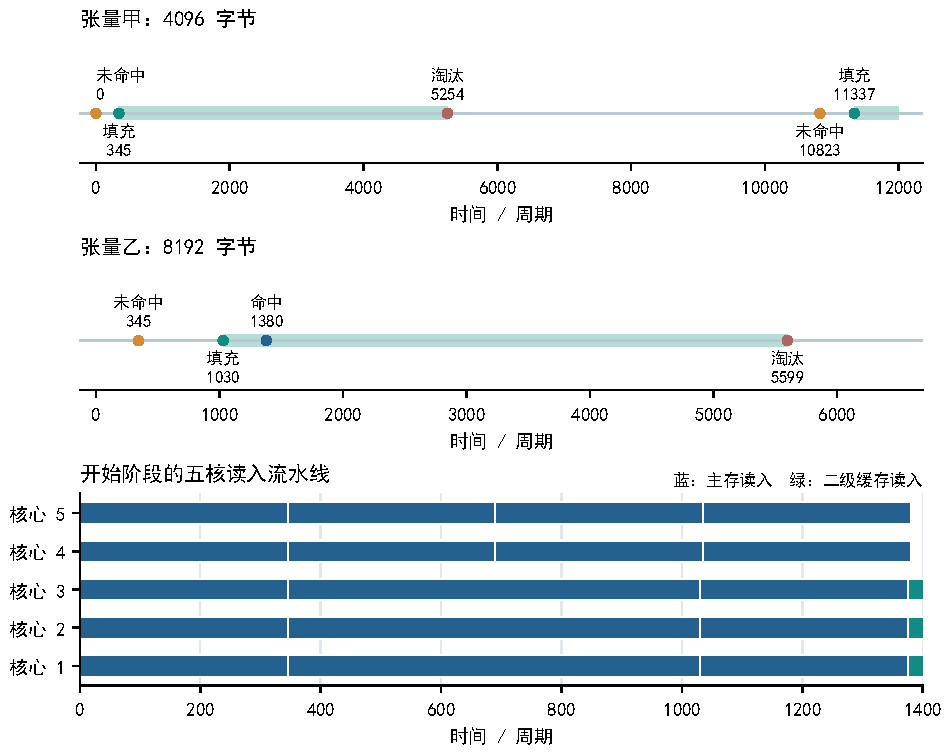
\includegraphics[width=\textwidth]{../求解/问题三/图片/q3_trace.pdf}
\caption{算例080的缓存驻留窗口与多核读入轨迹}\label{fig:q3_trace}
\end{figure}

张量甲在周期0的读取未命中，读入于周期345完成后进入缓存。周期5254的一次新填入将它淘汰。当另一核心在周期10823再次读入甲时，访问已落在这段驻留窗口之外，因此再次未命中。甲在周期11337重新填入，于周期15878再次被淘汰。周期21536的下一次读取仍未命中。

张量乙在周期345查询时未命中，于周期1030填充。周期1380的查询发生在其驻留期内，因而命中。此命中没有将乙移至队尾，周期5599它仍被后续填入淘汰。

图中最早的五个读请求均在周期0发射、周期345完成，显示共享 DDR 上的并发服务。对甲的 $4096$ B 请求，按每请求独占服务周期向上取整得到 $\lceil4096/60\rceil=69$ 周期。在这五个请求同时在途的区间，共享服务使其完成周期与 $5\times69=345$ 一致。

\subsubsection{固定方案的容量与带宽响应}
图~\ref{fig:q3_parameters} 的54个格点保持每张图的五核完整方案不变。算例080在容量 $262144$ B 下，L2 带宽依次为 $60$、$250$、$500$ B/周期时，总体任务执行时间依次为 $79170$、$80014$、$81744$ 周期。对应字节命中率为 $0.1960$、$0.1827$、$0.1680$。带宽提高后，命中率下降而总体任务执行时间上升，表明服务速度的改变伴随缓存访问状态变化。按照前述事件模型，服务完成时刻会影响后续请求发射、缓存填充与淘汰的相对次序。

容量响应也出现平台：算例080在带宽 $250$ B/周期下，容量从 $262144$ B 增至 $1048576$ B 时，周期由 $80014$ 降为 $63001$。继续增至 $4194304$ B，周期仍为 $63001$。算例044在容量 $1048576$ B 下，带宽从 $60$ 增至 $250$、$500$ B/周期，周期为 $50723$、$36208$、$44299$。这两组固定方案结果分别展示了容量增加后的平台和带宽增加后的周期回升，说明需要在完整事件执行中联合评价容量与带宽配置。

算例046五核同方案有L2和无L2的周期分别为 $49119$ 与 $95050$，周期比为 $1.9351$，字节命中率约为 $0.7132$。
